% FIG 6.4: preserve author topology; correct both plate interfaces.
% Elements: 1 laser, 2 plate, 3 gas cell, 4 semitransparent mirror.
% Main branches shown in book, not a full multiple-Fresnel-reflection tree.
\documentclass[border=4pt]{standalone}
% Shared style and physically derived plate geometry.
% User rules: curves > axes; labels large; italic component numbers;
% subfigure letters below; no invented measured values.
\usepackage{fontspec,unicode-math}
\setmainfont{Noto Serif}
\setsansfont{Noto Sans}
\setmathfont{STIXTwoMath-Regular.otf}
\usepackage{tikz}
\usetikzlibrary{arrows.meta,calc,decorations.markings,patterns.meta}
\pagestyle{empty}
\tikzset{
  opt/.style={draw=black,line width=.9pt,line cap=butt,line join=miter},
  axis/.style={draw=black,line width=.72pt,-{Latex[length=2.2mm,width=1.3mm]}},
  tick/.style={draw=black,line width=.72pt},
  beam/.style={draw=black,line width=1.18pt,line cap=butt,line join=miter},
  ray/.style={beam,postaction={decorate},decoration={markings,
       mark=at position .57 with{\arrow{Latex[length=2.3mm,width=1.35mm]}}}},
  pair/.style={beam,postaction={decorate},decoration={markings,
       mark=at position .32 with{\arrowreversed{Latex[length=2.3mm,width=1.35mm]}},
       mark=at position .72 with{\arrow{Latex[length=2.3mm,width=1.35mm]}}}},
  curve/.style={draw=black,line width=1.95pt,line cap=round,line join=round},
  curveDash/.style={draw=black,line width=1.65pt,dash pattern=on 3.6pt off 3.1pt,line cap=round},
  olabel/.style={font=\fontsize{14.5}{17.4}\selectfont,inner sep=1pt},
  oid/.style={font=\fontsize{14.5}{17.4}\selectfont\itshape,inner sep=1pt},
  opanel/.style={font=\fontsize{15}{18}\selectfont\itshape,inner sep=1pt},
}
% Planar faces parallel to tangent at PlateTilt; n points from face A to B.
% For incident horizontal ray in air: incidence = 90deg - PlateTilt.
% Index 1.5 and thickness are ILLUSTRATIVE drawing parameters, not book data.
\newcommand{\PlateParameters}[3]{%
  \def\PlateTilt{#1}\def\PlateThickness{#2}\def\PlateIndex{#3}%
  \pgfmathsetmacro{\PlateNormal}{\PlateTilt-90}%
  \pgfmathsetmacro{\Incidence}{90-\PlateTilt}%
  \pgfmathsetmacro{\RefractAngle}{asin(sin(\Incidence)/\PlateIndex)}%
  \pgfmathsetmacro{\InsideAngle}{\PlateNormal+\RefractAngle}%
  \pgfmathsetmacro{\InsideLength}{\PlateThickness/cos(\RefractAngle)}%
}
% #1 prefix, #2 entrance coordinate, #3 half-length of face.
\newcommand{\Plate}[3]{%
  \coordinate (#1A) at (#2);
  \coordinate (#1B) at ($(#1A)+(\InsideAngle:\InsideLength)$);
  \coordinate (#1Alow) at ($(#1A)+(\PlateTilt:-#3)$);
  \coordinate (#1Ahigh) at ($(#1A)+(\PlateTilt:#3)$);
  \coordinate (#1Blow) at ($(#1Alow)+(\PlateNormal:\PlateThickness)$);
  \coordinate (#1Bhigh) at ($(#1Ahigh)+(\PlateNormal:\PlateThickness)$);
  \draw[opt,fill=white] (#1Alow)--(#1Ahigh)--(#1Bhigh)--(#1Blow)--cycle;
}
% Author's conventional LASER symbol, not a two-mirror ray-traced cavity.
% Preserve two boundary lines. The external beam is anchored to Output.
% #1 prefix #2 left internal centre coordinate #3 width #4 number.
\newcommand{\Laser}[4]{%
  \coordinate (#1L) at (#2);
  \coordinate (#1Output) at ($(#1L)+(#3,0)$);
  \coordinate (#1Rinner) at ($(#1Output)+(30:-.10)$);
  \coordinate (#1Lt) at ($(#1L)+(60:.55)$);
  \coordinate (#1Lb) at ($(#1L)+(60:-.55)$);
  \coordinate (#1Rt) at ($(#1Output)+(120:.55)$);
  \coordinate (#1Rb) at ($(#1Output)+(120:-.55)$);
  \draw[opt,fill=white] (#1Lt)--(#1Lb)--++(150:.10)--($(#1Lt)+(150:.10)$)--cycle;
  \draw[opt,fill=white] (#1Rt)--(#1Rb)--++(210:.10)--($(#1Rt)+(210:.10)$)--cycle;
  % Side walls computed as intersections of horizontal edges and the faces.
  \pgfmathsetmacro{\LasLeftShift}{.30/tan(60)}
  \pgfmathsetmacro{\LasRightShiftTop}{(-.10-.30*cos(60))/cos(30)}
  \pgfmathsetmacro{\LasRightShiftBottom}{(-.10+.30*cos(60))/cos(30)}
  \draw[opt] ($(#1L)+(\LasLeftShift,.30)$)--($(#1Output)+(\LasRightShiftTop,.30)$);
  \draw[opt] ($(#1L)+(-\LasLeftShift,-.30)$)--($(#1Output)+(\LasRightShiftBottom,-.30)$);
  \node[oid] at ($(#1L)!.5!(#1Output)+(0,-.74)$) {#4};
}
% #1 prefix #2 entrance coordinate #3 length #4 number. No fill masks ray.
\newcommand{\GasCell}[4]{%
  \coordinate (#1In) at (#2);
  \coordinate (#1Out) at ($(#1In)+(#3,0)$);
  \draw[opt] ($(#1In)+(0,-.52)$) rectangle ($(#1In)+(.14,.52)$);
  \draw[opt] ($(#1Out)+(-.14,-.52)$) rectangle ($(#1Out)+(0,.52)$);
  \draw[opt] ($(#1In)+(.14,.34)$)--($(#1Out)+(-.14,.34)$);
  \draw[opt] ($(#1In)+(.14,-.34)$)--($(#1Out)+(-.14,-.34)$);
  \node[oid] at ($(#1In)!.5!(#1Out)+(0,-.80)$) {#4};
}
% A real turning mirror: incident point belongs to the reflecting face.
% The shaded support is strictly on the other side of that face.
\newcommand{\TurnMirror}[2]{%
  \coordinate (#1Lo) at ($(#1)+(45:-.57)$);
  \coordinate (#1Hi) at ($(#1)+(45:.57)$);
  \path[pattern={Lines[angle=135,distance=2.1pt,line width=.35pt]}]
        (#1Lo)--(#1Hi)--++(-45:.13)--($(#1Lo)+(-45:.13)$)--cycle;
  \draw[opt] (#1Lo)--(#1Hi)--++(-45:.13)--($(#1Lo)+(-45:.13)$)--cycle;
  \node[oid] at ($(#1)+(.62,-.34)$) {#2};
}

\begin{document}
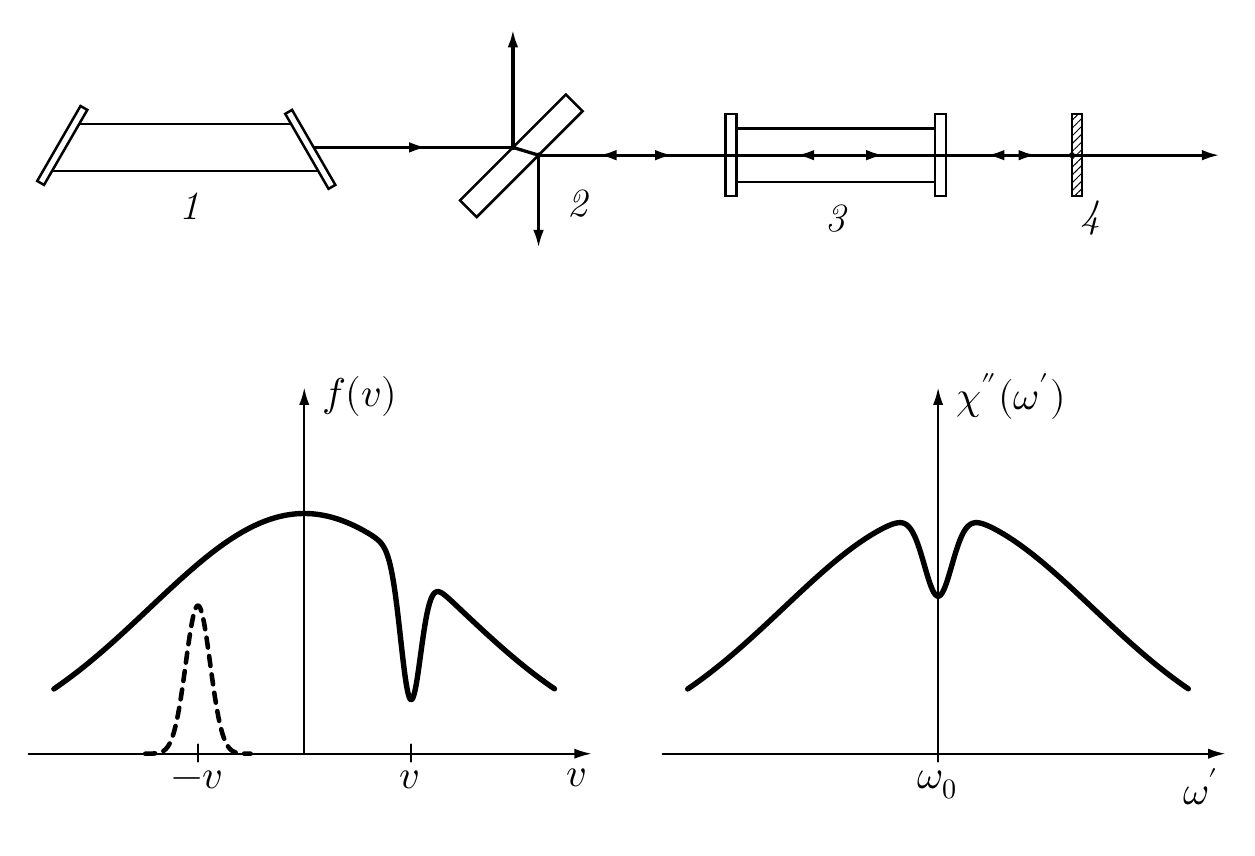
\begin{tikzpicture}[x=1cm,y=1cm,line cap=round,line join=round]
\PlateParameters{45}{.30}{1.50}
\coordinate (Entrance) at (6.30,8.50);
\Plate{P}{Entrance}{.95}
\coordinate (LaserBase) at (.62,8.50);
\Laser{L}{LaserBase}{3.15}{1}
\draw[ray] (LOutput)--(PA);
% PA/PB are the geometrically calculated intersections with the two
% parallel faces; no ray originates from an unrelated decorative point.
\draw[beam] (PA)--(PB);
\fill (PA) circle[radius=.035cm];
\fill (PB) circle[radius=.035cm];
\draw[beam,-{Latex[length=2.3mm,width=1.35mm]}] (PA)--++(0,1.50);
\draw[beam,-{Latex[length=2.3mm,width=1.35mm]}] (PB)--++(0,-1.18);
\node[oid] at ($(PB)+(.50,-.62)$) {2};
\coordinate (CellIn) at (9.0,0 |- PB);
\GasCell{C}{CellIn}{2.80}{3}
\coordinate (Mirror) at (13.40,0 |- PB);
\coordinate (AfterMirror) at ($(Mirror)+(.13,0)$);
\path[pattern={Lines[angle=45,distance=2.0pt,line width=.35pt]}]
       ($(Mirror)+(0,-.52)$) rectangle ($(AfterMirror)+(0,.52)$);
\draw[opt] ($(Mirror)+(0,-.52)$) rectangle ($(AfterMirror)+(0,.52)$);
\node[oid] at ($(Mirror)+(.23,-.80)$) {4};
\draw[pair] (PB)--(CIn);
\draw[pair] (CIn)--(COut);
\draw[pair] (COut)--(Mirror);
% Reflection and transmission meet at the real semitransparent mirror face.
\fill (Mirror) circle[radius=.038cm];
\draw[beam] (Mirror)--(AfterMirror);
\draw[beam,-{Latex[length=2.3mm,width=1.35mm]}] (AfterMirror)--++(1.75,0);
\node[opanel] at (7.90,6.73) {а};
% Spectra retained as schematic author-based contours; not new data.
\begin{scope}[shift={(.15,.80)}]
  \draw[axis] (0,0)--(7.15,0);
  \draw[axis] (3.50,0)--(3.50,4.65);
  \node[olabel,anchor=west] at (3.69,4.54) {$f(v)$};
  \node[olabel,anchor=north east] at (7.12,-.15) {$v$};
  \draw[curve,samples=500,domain=-3.18:3.18,smooth]
    plot ({3.50+\x},{3.05*exp(-(.36*\x)^2)-1.72*exp(-((\x-1.35)/.18)^2)});
  \draw[curveDash,samples=200,domain=-.67:.67,smooth]
    plot ({2.15+\x},{1.88*exp(-((\x)/.22)^2)});
  \foreach \x in {2.15,4.85}{\draw[tick] (\x,-.10)--(\x,.12);}
  \node[olabel,anchor=north] at (2.15,-.18) {$-v_{\mathrm{рез}}$};
  \node[olabel,anchor=north] at (4.85,-.18) {$v_{\mathrm{рез}}$};
  \node[opanel] at (3.55,-.91) {б};
\end{scope}
\begin{scope}[shift={(8.20,.80)}]
  \draw[axis] (0,0)--(7.15,0);
  \draw[axis] (3.50,0)--(3.50,4.65);
  \node[olabel,anchor=west] at (3.69,4.54) {$\chi''(\omega')$};
  \node[olabel,anchor=north east] at (7.12,-.15) {$\omega'$};
  \draw[curve,samples=500,domain=-3.18:3.18,smooth]
    plot ({3.50+\x},{3.05*exp(-(.36*\x)^2)-1.05*exp(-((\x)/.25)^2)});
  \draw[tick] (3.50,-.10)--(3.50,.12);
  \node[olabel,anchor=north] at (3.50,-.18) {$\omega_0$};
  \node[opanel] at (3.55,-.91) {в};
\end{scope}
\end{tikzpicture}
\end{document}
